%% -*- coding: utf-8; -*-

\documentclass[phd,american]{ThesisPUC}

%---------- Math ----------%
\usepackage{amsmath}
\usepackage{amssymb}
\usepackage{mathtools}
\usepackage{bbm}
\usepackage{ulem}
%---------- Floting ----------%
\usepackage{float}
% ---------- References ----------%
%\usepackage[sort&compress,round,comma,numbers]{natbib}
%\usepackage{natbib}
%---------- Algorithm ----------%
\usepackage[algosection, algoruled]{algorithm2e}
%---------- Tables ----------%
\usepackage{multicol}
\usepackage{booktabs}
%---------- TiKz ----------%
\usepackage{threeparttable}
\usepackage{standalone}
\usepackage{xcolor}
\usepackage{tikz}
\usepackage{psfrag,epsf}
%\usepackage{todonotes}
\usepackage{multirow}
\usepackage{listings}
\usepackage{soul}
%----------citation------------%
%\usepackage{apacite}

%-----------color-----------------%
\definecolor{dkblue}{rgb}{0,0,.6}
\definecolor{turquoise}{rgb}{0.25,0.87,0.82}
\definecolor{dkgreen}{rgb}{0,0.6,0}
\definecolor{dkred}{rgb}{0.7,0,0}
\definecolor{indigo}{rgb}{0.294, 0, 0.51}
\definecolor{cyan}{rgb}{0, 0.70, 0.70}
\definecolor{gray}{rgb}{0.5,0.5,0.5}
\definecolor{mauve}{rgb}{0.58,0,0.82}
\definecolor{black}{rgb}{0,0,0}

\newcommand{\pmendes}[1]{\color{red}\textbf{paulo says: }#1\color{black}}


%\pagestyle{plain}


%Para o código em EPL
\lstdefinestyle{EPLStyle}{
  numbers=left,
  numberstyle=\footnotesize\ttfamily,
  language=SQL,
  frame=tblr,
  aboveskip=0mm,
  belowskip=3mm,
  showstringspaces=false,
  columns=flexible,
  basicstyle={\small\ttfamily},
  numberstyle=\tiny\color{gray},
  keywordstyle=\color{blue},
  commentstyle=\color{gray},
  stringstyle=\color{dkgreen},
  breaklines=true,
  breakatwhitespace=true,
  tabsize=3,
  %Adiciona as keywords específicas da EPL Esper
  morekeywords={after, at, context, current_timestamp,  define, distinct, every, first, grouping, grouping_id, hour, hours, initiated, inner, instanceof, irstream, is, istream, last, match_recognize,  measures, min, minute, minutes, microsecond, microseconds, millisecond, milliseconds, msec, new, offset, output, partition, pattern, rstream, sec, second, seconds, sets, some, snapshot, sql, start, terminated, then, until, usec, using, variable, weekday, when, while, window, schema},
%
  frameround=tttt,
}

\graphicspath{{images/}}

% ---------- Cover ----------%
% Adjust the advisor's title according to gender(Prof. or Prof$^{\text{a}}$.)
\author{Paulo Renato Conceição Mendes}
\authorR{Mendes, Paulo Renato Conceição}
\advisor{Sérgio Colcher}{Prof.}
\advisorR{Colcher, Sérgio}

% This thesis will use colored figures, this goes in the catalographic sheet
\usecolour{true}
\title{Spatiotemporal Localization of Actors   in Video/360-Video and its Applications}

\titleuk{Spatiotemporal Localization of Actors in Video/360-Video and its Applications}

\day{27$^{th}$}
\month{July}
\myyear{2021}

% CDD is the registry number of the area, given by the library. Our area (informatics) is 004.
\city{Rio de Janeiro}
\CDD{004}
\department{Informática}
\program{Informática}
\school{Centro Técnico Científico}
\university{Pontifícia Universidade Católica do Rio de Janeiro}
\uni{PUC-Rio}

%---------- Jury ----------%

% Internal jury members are declared with \jurymember{name}{title}{department}{university}
% external jury members are declared with \extjurymember{name}{title}{university}
\jury{
  \jurymember{Alberto Barbosa Raposo}{Prof.}{Departamento de Informática}{PUC-Rio}
  \extjurymember{Roberto Gerson de Albuquerque Azevedo}{Dr.}{Departamento de Ciência da Computação -- ETH Zurich}
  %\extjurymember{Jury 1}{Dr.}{Uni}
  % The person below is mandatory.
  % \schoolhead{Márcio da Silveira Carvalho}{Prof.}
}

%---------- Front letters ----------%
\resume
{
Bachelor's degree in Computer Science at Federal University of Maranhão (UFMA) in 2019.
}

\acknowledgment
{
\noindent
Thanks to my advisor Prof. Sérgio Colcher for his guidance and support in this journey.
Thanks to my family for the endless support.
Thanks to my friends from TeleMídia Lab, for their friendship and support. To all colleagues, faculty and staff of the PUC Rio Department of Informatics for the fellowship, learning and support.
This study was financed in part by the Coordenação de Aperfeiçoamento de Pessoal de Nível Superior - Brasil (CAPES) - Finance Code 001.
}


% Workaround for keywords. The keywords in the catalographic sheet must be separated by dots, while the ones shown in the abstract must be separated by semi-colons.
% Thats why we have two commands for each language: \keywords declares the keywords for the catalographic sheet, while \keywordsabstract declares the ones for the abstract.
\keywords
{
  \key{Clusterização}
  \key{Reconhecimento Facial}
  \key{Recomendação}
  \key{Vídeo 360}
  
  
}

\keywordsabstract
{
  \key{Clusterização;}
  \key{Reconhecimento Facial;}
  \key{Recomendação;}
  \key{Vídeo 360.}
}

\keywordsuk
{

  \key{Clustering}
  \key{Face Recognition}
  \key{Recommendation}
  \key{360-Video}
}

\keywordsabstractuk
{
  \key{Clustering;}
  \key{Face Recognition;}
  \key{Recommendation;}
  \key{360-Video.}
}

\abstract{
  A disseminação atual da IoT aumenta a implantação de soluções de processamento de fluxo de dados para monitorar e controlar elementos do mundo real. Uma dessas soluções é o Processamento de Eventos Complexos (CEP). Inicialmente, um único computador ou cluster concentraria toda a execução do CEP. No entanto, a execução centralizada do CEP não é ideal para lidar com o alto volume, velocidade e volatilidade dos fluxos de dados dos sensores IoT. Em vez disso, as aplicações CEP devem criar e decentralizar o processamento de eventos CEP, de preferência tendo agentes CEP na nuvem e em dispositivos na borda. Além disso, tão importante quanto a descentralização, é decidir como o processamento será dividido entre esses dispositivos. Dito isso, estar ciente do contexto atual de cada dispositivo, por exemplo, sua localização e sensores disponíveis, pode ajudar a coletar e (parcialmente) processar os dados em dispositivos próximos ao local onde os dados foram produzidos. Este trabalho apresenta uma plataforma de CEP distribuído com ciência de contexto chamada Global CEP Manager (GCM). GCM é um serviço do middleware ContextNet que oferece suporte à implantação e ao rearranjo dinâmico de consultas CEP baseados em contexto para motores CEP em execução na nuvem, em dispositivos na borda estacionários e M-Hubs, que são dispositivos na borda móveis do ContextNet. O GCM usa o ContextMatcher, que também faz parte deste trabalho. ContextMatcher é um módulo para aplicações ContextNet que permite a entrega de mensagens para nós cujo contexto esteja de compatível com um determinado conjunto de características contextuais.
}

\abstractuk{
  The current dissemination of IoT increases the deployment of stream processing solutions for monitoring and controlling elements of the real world. One of those solutions is Complex Event Processing (CEP). Initially, a single computer/cluster would concentrate all the CEP execution. However, a centralized execution of CEP is not suitable for coping with the high volume, velocity, and volatility of IoT sensors’ data streams. Instead, applications using CEP should deploy a distributed CEP Event Processing Network, preferably having CEP agents both in the cloud and at edge devices. Also, deciding the arrangement used to split the processing among these tiers and their devices can be just as important. That said, being aware of each of the devices’ current context, for instance, their location and available sensors, can help to collect and (partially) process the data on devices close to the data’s production site. This work presents a context-aware distributed CEP platform called Global CEP Manager (GCM). GCM is a service of the ContextNet middleware that supports the context-based deployment, and dynamic rearrangement of CEP queries to CEP engines executing in the cloud, stationary edge devices, and  M-Hubs, which are ContextNet’s mobile edge devices. GCM uses the ContextMatcher, which is also part of this work. ContextMatcher is a module for ContextNet applications that enables the delivery of messages for nodes that match a specified set of contextual requirements.
}


% WARNING
% The epigraph, if present, must come before the first chapter, always.
% There is a list of abreviations (abrevs.tex) which is included automatically in the ThesisPUC.cls, and is optional, comment the %% -*- coding: utf-8; -*-

\begin{thenotations}
\renewcommand{\arraystretch}{1.5}
  \noindent
  \begin{tabular}{ll}

CNN -- Convolutional Neural Network\\
FDDB -- Face Detection Data set and Benchmark\\
FOV -- Field of View\\
FRPC -- Face Recognition Prize Challenge\\
GTP -- Ground Truth Positives\\
HMD -- Head-Mounted Display\\
HOG -- Histogram of Oriented Gradients\\
HTML -- HyperText Markup Language\\
HUD -- Heads-up Display\\
IARPA -- Intelligence Advanced Research Projects Activity\\
IJB -- IARPA Janus Benchmark-B\\
LFW -- Labeled Faces in the Wild\\
MAP -- Mean Average Precision
MOOC -- Massive Open Online Course\\
MTCNN -- Multitask Cascaded Convolutional Networks\\
NAN -- Neural Aggregation Network\\
NCL -- Nested Context Language\\
NMS -- Non-Maximum Suppression\\
PIP -- Picture-in-Picture\\
SMIL -- Synchronized Multimedia Integration Language\\
SRT -- SubRip Subtitle Format\\
VR -- Virtual Reality\\
VTE -- Virtual Teaching Environment\\
XML -- Extensible Markup Language\\

  \end{tabular}

\end{thenotations} line if you do not wish to included it.
% Rationale: In the original template, the list of abreviations came before the epigraph, which caused problems with the university library, thus I've included it in the cls file.
% TODO: Declare a boolean option in the ThesisPUC.cls class in order to selectively include the abreviations list.

%%%%%%%%%%%%%%%%%%%%%%%%%%%%%%%%%%%%%%%%%%%%%%%%%%%%%%
\begin{document}

%%% -*- coding: utf-8 -*-
\newpage

\chapter{Introduction}
\label{chap:introduction}

In recent years, the popularity of platforms for the storage and transmission of video content has stimulated the production of a massive volume of video data, establishing new habits, and leveraging new applications with innovative forms of consumption of this kind of information. Just as an indication of this huge production (and consumption) of data, we mention that, in 2019, for example, more than one billion hours of YouTube videos were watched per day.\footnote{https://kinsta.com/blog/youtube-stats/}


Generating metadata with (i) the identity information of actors present, (ii) the temporal determination of the intervals in which each of these actors is present, and (iii) their spatial localization in each of the frames along these intervals can facilitate video indexing, retrieval, recommendation and a series of other tasks which might enhance the way people interact and consume all this video data. Besides the identification, (ii) and (iii) together are what we call \textit{Spatiotemporal Localization}. 

In this dissertation, we investigate a method for the spatiotemporal localization of actors in videos. Our expected contribution is two-fold: 
\begin{enumerate}
\item we propose a core process for the spatiotemporal localization in which we take advantage of face detection, embeddings, and clustering methods to group similar faces (presumably from the same actors) along with the frames, and \item we further explore, propose and investigate the innovative application of this localization in three different practical and important tasks: \emph{Video Face Recognition}, \emph{Educational Video Recommendation}, and \emph{Subtitles Positioning in 360-video}.  
\end{enumerate}

The common core of this dissertation relies on its first part, in which we describe a \textit{Video Face Clustering} method for the spatiotemporal localization of actors. We describe its process composed of: \textit{frame extraction}, \textit{face detection}, \textit{embeddings generation} and \textit{clustering}. 

Based on this \emph{Video Face Clustering} method, we investigate three chosen applications in which we explore novel approaches, all of them enabled by that common method of localization and its benefits. 

The first application, that of \emph{Video Face Recognition}, has been attracting the attention of researchers for more than two decades. Since the deep learning boom, face detection and recognition performance have greatly improved in terms of both speed and accuracy~\cite{masi2018deep}. Nowadays, face recognition systems are used in many areas such as video surveillance and security systems, video analytics systems, smart shopping, automatic face tagging in photo collections, investigative tools that search for identities in social networks based on face images, and in thousands of other applications in our daily lives.

In our work, we propose a \textit{cluster-matching-based approach} for \emph{Video Face Recognition} where clustering is used to group faces in both the face dataset and in the target video. This method was motivated (and made possible) mainly by the characteristics of our core \emph{Video Face Clustering} method. Its main benefit is that classes (which represent different actors) do not have to be previously known, so the effort spent with annotations is significantly reduced --- as it is done over clusters instead of single images. Consequently, face recognition becomes a task of comparing clusters from the dataset with the ones extracted from images or video sources. Therefore, our approach is easily scalable and can be used to automatically generate video metadata.

The second application, that of \emph{Educational Video Recommendation}, may be considered as one of a more general class of applications referenced as \textit{recommendation system applications} and was motivated by a shift of paradigms that we have been observing in recent years. The traditional paradigm of classroom courses, centered on the physical presence of a teacher, has been gradually giving space to online and hybrid courses, which enables the emergence of VTEs (Virtual Teaching Environment) and MOOCs~(\textit{Massive Open Online Courses}).
If, on the one hand, the abundance of educational videos can contribute to and facilitate learning, on the other hand, it also makes it challenging to discover and access some specific content of interest~\cite{dias2017approach}.
This issue is usually addressed by a proactive user search (using queries, for example), or by automatic recommendations made by specialized systems.


In general, current video recommendation methods are heavily dependent on textual information from the video, such as labels (\textit{i.e.} keywords)~\cite{mahajan2015optimising,omisore2014personalized}, or automatically generated captions \cite{barrere2020utilizaccao} from the lecturer speech. These systems face problems such as errors introduced by manually inserted labels or by imprecise speech recognition.
In this work, we propose an additional feature to enhance the recommendation of educational video content which is based on actors~(in this specific case, lecturers) presence. To do that, again we take advantage of our core \emph{Video Face Clustering} method. More precisely, we detect lecturers in a video taken as a reference and perform a clustering based on the face of these lecturers in different videos. Given these clusters, we extract their \textit{centroids} and perform another clustering step for creating a relationship between videos that share the presence of the same lecturers. Finally, we rank the recommended videos based on the amount of time the referenced lecturers were present.
A particular benefit of this approach is that it can be done without supervision, allowing for new videos to be automatically analyzed.

Our third application (\emph{Subtitles Positioning in 360-Video}) was motivated by the recent popularization of omnidirectional cameras and Head-Mounted-Displays (HMDs) that increased the amount of 360-video content available. Omnidirectional videos are spherical visual signals that allow the viewer to look around a full 360-degree view of a scene from a specific point.

Several people use subtitles when consuming audiovisual media, and these subtitles are important in contributing to the understanding of the video content \cite{brown_subtitles_2017}. Some people choose to consume videos muted \cite{hughes_disruptive_2019}. Additionally, the work of \cite{hayati2011effect}, as referenced in \cite{hughes_disruptive_2019}, shows that consumers are more likely to watch videos entirely if they have subtitles presented with them. In traditional 2D videos, static subtitles are commonly used and they are usually placed at a fixed position, most commonly at the bottom-center of the screen \cite{rothe_dynamic_2018}.
Different from traditional 2D videos, subtitles positioning in 360-videos is challenging because it involves both temporal and spatial domains \cite{agullo2019making}, and there is no fixed ``bottom-center" of the screen \cite{brown_subtitles_2017}. Most current solutions rely on positioning subtitles either statically to the viewer or at a fixed position in the 360-degree environment. 
In this work, we adapt and apply our current solution for the spatiotemporal localization of actors to the 360-video domain. By doing that, we intend to use this localization for positioning subtitles close to the actors in the 360-video.

The remainder of this dissertation proposal is structured as follows. 
In Chapter \ref{chap:related}, we discuss some works related to the core method of our dissertation and each of the applications we investigate.
In Chapter \ref{chap:video_face_clustering}, we define our approach for spatiotemporal localization of actors, which is our core method.
The following three chapters contain the applications in which we investigate the applicability of this method.
The first application, that of \emph{Video Face Recognition}, is described in Chapter \ref{chap:face_recognition}.
In Chapter \ref{chap:educational_recommendation}, we present our application of \emph{Educational Video Recommendation}.
Our last application, that of \emph{Subtitles Positioning in 360-video}, is described in Chapter \ref{chap:subtitles_positioning}. Finally, in Chapter \ref{chap:conclusions}, we conclude this dissertation and point to possible future work.
%%%% -*- coding: utf-8 -*-
\newpage

\chapter{Background}
\label{chap:background}
%%% -*- coding: utf-8 -*-
\newpage

\chapter{Related Work}
\label{chap:related}

In this chapter we make a brief review of the works related to ours. Section \ref{sec:spatiotemporal} contains works related to the core method of this word. The next three sections describe works related to the applications we propose based on our core method.

\section{Spatiotemporal Localization of Actors}
\label{sec:spatiotemporal}


The task of detecting and tracking actors in video has been the focus of many researches. In early 2004, \cite{facetracking_2} used an illumination invariant approach for face detection combined with a tracking mechanism performed by means of continuous detections. \cite{face_tracking} addressed the problem of tracking faces in noisy videos using a tracker that adaptively builds a target model reflecting changes in appearance, typical of a video setting. This kind of approaches does not perform well in the task of spatiotemporal localization of actors because they can only track them when they are continuously present on the video. Differently, the approach we use, which is based on clustering, does not require the actors to be continuously present on the video.

More similar to ours, recent works have investigated the use of clustering for grouping faces of actors in video and, consequently, providing the spatiotemporal localization of them. \cite{video_face_clustering} propose Ball Cluster Learning~(BCL), a supervised approach to carve the embedding space into balls of equal size, one for each cluster. The radius of such ball is translated to a stopping criterion for iterative merging algorithms. \cite{self_supervised} propose a self-supervised Siamese network for video face clustering that can also be used in scenarios where tracks of actors are not available, such as image collections. The approach we use can also be applied to image collections, as further explained in Section \ref{chap:face_recognition}, but it differs in the sense that we use pre-trained CNNs and traditional clustering algorithms for performing this task. 

It is worth mentioning that, in this dissertation, we do not intend to directly compare or propose a better method for the task of spatiotemporal localization of actors than the existing ones. Instead, we intend to investigate in what extent our method opens up novel approaches for the three chosen applications and the benefits that can be achieved with our approach.

\section{Video Face Recognition}
\label{sec:video_face}

Many methodologies have been proposed for Video Face Recognition, most commonly relying on comparing selected facial features of a given image with features of faces within a database.
%%
Using only one sample reference image of a person's face for the comparison may result in classification errors due to factors related to variations in lighting, image resolution, angle, etc.~\cite{598229}.
%%
To overcome this problem, some face recognition approaches use multiple face samples for comparison. However, this strategy does not scale well as the complexity is a function of the number of samples.
%%
Other approaches treat the face recognition task as a classification problem~\cite{dadi2016improved, ghosal}, where a classifier model learns rules to assign faces to previously known classes within a dataset, where each class corresponds to one person.
%%
Nonetheless, this kind of approach does not deal well when new classes are incorporated because of the need to retrain the classification models.
%%
Moreover, when dealing with video, these kinds of methods have to be applied to each frame, again increasing the complexity.


Traditional deep learning models for face recognition such as DeepFace~\cite{taigman2014deepface} and DeepID~\cite{sun2014deep} use a CNN with fully-connected layer output to produce a representation of high-level features (face embeddings) from an input image, followed by a softmax layer to indicate the identity of classes. Other approaches, such as FaceNet~\cite{schroff2015facenet}, can directly measure the similarity among faces using euclidean space. Inspired by DeepID, this model uses the \textit{triplet loss} as the loss function to estimate similarity to one character's face to a  collection of other faces. Triplet loss improves the accuracy of the  CNN output by minimizing the euclidean distance between the anchor and the positive (face of the same identity) while maximizing the distance between the anchor and the negative (face of another identity). In this work, we evaluated different pre-trained CNN backbones on VGGFace2 dataset~\cite{cao2018vggface2} to generate the face embeddings. This model is the state-of-the-art\footnote{https://paperswithcode.com/paper/vggface2-a-dataset-for-recognising-faces} in the face verification task on the IJB-B dataset~\cite{whitelam2017iarpa}. 


Proprietary systems for face recognition and matching are widely used by social network platforms. For instance, Facer~\cite{hazelwood2018applied} is Facebook's face detection and recognition framework. Given a photograph, it first detects all the faces. Then, it runs a  deep model to determine the likelihood of that face belonging to one of the top-N user friends. This allows  Facebook to suggest which friends the user might want to tag within the uploaded photographs. FindFace\footnote{https://findface.br.aptoide.com/app} is an app that matches photos to profile pictures on VKontakte,\footnote{https://vk.com/} a Russian social networking website similar to Facebook. FindFace uses a deep model developed by NTech Lab that won the \textit{2017 IARPA Face Recognition Prize Challenge} (FRPC)~\cite{grother20172017}  in two nominations out of three (“Identification Speed” and “Verification Accuracy”). Similarly, our method can detect faces in videos and automatically recognize their identities by a clustering-based algorithm that uses a knowledge base with the faces pre-identified as a reference; however, a comparison with such methods was not possible due to access restrictions.

Some recent works are focused on video face recognition. Pena \textit{et al.}~\cite{globofacestream} proposed a face recognition system to detect characters within videos, called~\textit{Globo Face Stream}. Their method uses a Histogram of Oriented Gradients (HOG) feature combined with a linear classifier to detect faces. Next, they use  FaceNet to generate the embeddings, followed by the euclidean distance calculus to measure the similarity among faces. Yang \textit{et al.}~\cite{yang2017neural} proposed a deep network for video face recognition called NAN (Neural Aggregation Network). They use a CNN to generate the embeddings, followed by an aggregation module that consists of two attention blocks which adaptively aggregate the feature vectors to form a single feature inside the convex hull spanned by them. Rao \textit{et al.}~\cite{rao2017attention} proposed a method for video face recognition based on attention-aware deep reinforcement learning. They formulated the process of finding the attention of videos as a Markov decision process and training the attention model without using extra labels. Unlike existing attention models, their method takes information from both the image space and the feature space as the input to make use of face information that is discarded in the feature learning process. Sohn \textit{et al.}~\cite{sohn2017unsupervised} proposed an adaptative deep learning framework for image-based face recognition and video-based face recognition. Given an embedding generated by a CNN, their framework adaptation is achieved by (1) distilling knowledge from the network to a video adaptation network through feature matching, (2) performing feature restoration through synthetic data augmentation, and (3) learning a domain-invariant feature through an adversarial domain discriminator. 

Like~\cite{globofacestream, yang2017neural, rao2017attention, sohn2017unsupervised}, our method uses a CNN to generate face embeddings from face images, with the difference that it uses an unsupervised cluster-based method to compare the similarity among face datasets and faces extracted from videos. Also, our approach can detect faces that do not have an identity registered in the face dataset with excellent performance.

\section{Educational Video Recommendation}
\label{sec:recommendation}

Recommendation mechanisms are usually based on two methods: \textit{collaborative filtering} and \textit{content-based filtering}. 
In collaborative filtering, the system groups users based on their common interest on items, using users' preferences, rates, purchases or accesses to those items. With this approach, 
knowledge about the item's content is not needed; the recommendation is purely based on the relationship between users and items.  The content-based filtering, differently, requires items' description; similar items are the ones recommended to the user. Our approach fits in the latter category. In the remainder of this subsection, we describe some works devoted to the task of general \emph{Video Recommendation}. Moreover, we give a especial focus on works that share our goal of investigating \emph{Educational Video Recommendation}.

The way people watch and consume video content has been changing in the last years, moving from the traditional linear content transmission of  televisions to streaming platforms. These platforms allow users to consume video content on demand. Some examples of such platforms are YouTube,\footnote{\url{https://youtube.com}} Netflix,\footnote{\url{https://netflix.com}} Prime Video\footnote{\url{https://primevideo.com}} and Globoplay.\footnote{\url{https://globoplay.globo.com}}. In such platforms, users can retrieve video content through actively searching for their content of interest or can be presented with recommendations of such content, from which they may select one to watch. 
%%
In this scenario, recommendations play a fundamental role in content promotion inside these platforms. It is common to use a collaborative filtering approach for recommending content to a specific user, and this kind of approach does not use any information about the content of the video. It is useful and shows good results when both the video content and user have a consumption history stored~\cite{ferreira2020investigating}. 
%%
However with new titles being uploaded daily to these platforms associated with their expanding user base, collaborative filtering does not perform well when with these new titles and users due to the lack of consumption history~\cite{suvash14social}. For that reason, our work is based on content-filtering,

Taking into consideration the problem of video recommendation with recently added videos, \cite{li2017study} propose a content-based video recommendation approach by taking advantage of CNNs to alleviate the cold-start problem. The authors represent video data with features from audio, images and meta-data from the video content and use such content to recommend videos in a streaming platform. In \cite{lee2017large}, the authors model recommendation as a video content bases similarity learning problem, and learn deep video embeddings trained to predict video relationships identified by a co-watch-based system but using only visual and audio content. \cite{han2016dancelets} proposes to take advantage of the intrinsic motion information in dance videos to solve the video recommendation problem. The authors aim at recommending dance videos based on a mid-level action representation called Dancelets and use a random forest-based index to achieve fast matching of styles and to generate the final recommendation ranking of videos. Similar to \cite{li2017study} and \cite{lee2017large}, we take advantage of CNNs for extracting content from the videos and perform recommendations. Differently, our work focuses on recommending videos sharing the presence of the same actors. Similar to \cite{han2016dancelets}, our work also does not require any metadata from the video, it is solely based on the video content.

Regarding \textit{Educational Video Recommendation}, most works perform analyses and comparisons using the video textual description or speech recognition performed on them. Omisore \textit{et. al.} \cite{omisore2014personalized}, for example, propose combining \textit{fuzzy} techniques to recommend books with content suitable for students based on their reading histories in a digital library, while Mahajan \textit{et. al.} \cite{mahajan2015optimising} propose, given a reference video,  mining social media, and web for suggesting links for a student to visit.
Moreover, Barrére \textit{et. al.}
~\cite{barrere2020utilizaccao} use texts from speech recognition to create recommendations.
These works are only based on textual characteristics~(or content converted to it) for performing recommendations.
Our work focuses on using a visual part of the video, more precisely the presence of actors.


\section{Subtitles Positioning in 360-video}
\label{sec:subtitles}

We searched for works that used strategies for subtitles positioning and extracted the strategies they presented, also described as subtitling behaviour~\cite{brown_subtitles_2017}, in 360-degree videos. Then, we merged the similar strategies and divided them into three main categories: \emph{screen-referenced subtitles}, \emph{world-referenced subtitles} and \emph{dynamic subtitles}. Each of these categories are described in Subsections \ref{subsec:screen_referenced}, \ref{subsec:world_referenced}, and \ref{subsection:dynamic_subtitles} respectively. Table \ref{tab:catalog} contains a summary about the strategies in each category, their advantages and disadvantages.
%%

\begingroup
%\renewcommand{\baselinestretch}{1.5}
\begin{table}[!ht]
\footnotesize
\caption{Subtitles positioning strategies catalog for 360-degree video}
\label{tab:catalog}
\hspace{-1em}
\begin{tabular}{@{}llll@{}}
\toprule
\textbf{Category}                                               & \textbf{Strategy}  & \textbf{Advantages}                                                                                    & \textbf{Disadvantages}                                                                                         \\ \midrule
\multicolumn{1}{c}{\multirow{6}{*}{\textbf{Screen-Referenced}}} & Static-Follow      & \begin{tabular}[c]{@{}l@{}}easy to locate;\\ freedom of\\ movement;\\ most common\\ strategy;\end{tabular} & issues with nausea;                                                                                            \\ \cmidrule(l){2-4} 
\multicolumn{1}{c}{}                                            & Lag-Follow         & \begin{tabular}[c]{@{}l@{}}issues with\\nausea mitigated\\ in comparison\\to static-follow;\end{tabular} & may cause rereading;                                                                                           \\ \midrule
\multirow{2}{*}{\textbf{World-Referenced}}                      & Repeated Subtitles & \begin{tabular}[c]{@{}l@{}}comfort;\\ could be\\``burnt-in'' the video;\end{tabular}                    & \begin{tabular}[c]{@{}l@{}}may cover\\important content;\\ may be confusing;\\ not always visible;\end{tabular} \\ \cmidrule(l){2-4} 
                                                                & Appear             & \begin{tabular}[c]{@{}l@{}}comfort;\\ subtitles can\\be ``dismissed";\end{tabular}                      & \begin{tabular}[c]{@{}l@{}}may be positioned in\\ spurious locations;\\ not always visible;\end{tabular}       \\ \midrule
\textbf{Dynamic}& Speaker-Following  &\begin{tabular}[c]{@{}l@{}}  help in speaker\\identification; 
\end{tabular}& not always visible;                                                                                            \\ \bottomrule
\end{tabular}
\end{table}
\endgroup

\subsection{Screen-Referenced Subtitles}
\label{subsec:screen_referenced}

In this category, the subtitles are positioned taking the screen as reference, which can also be the viewport in a HMD. The subtitles basically follow the user's view and can be seen at any instant of time. We have identified two strategies following this category: \emph{static-follow} and \emph{lag-follow}. Each of these strategies are describe in Subsections \ref{subsubsec:static_follow} and \ref{subsubsec:lag_follow}, respectively.

\subsubsection{Static-Follow}
\label{subsubsec:static_follow}

When defining the \emph{static-follow} strategy, \cite{brown_subtitles_2017} argue that it is a common behaviour for showing information in Virtual Reality~(VR) experiencies, as part of a ``head-up display'' (HUD). A HUD typically displays graphics that are fixed in front of the viewer at all times regardless of their posture and pose in a VR environment. Figure \ref{fig:static_follow} shows this strategy, which uses the aforementioned HUD mechanic. In this strategy, the subtitles are shown to the viewer as if they were static relative to their head, by following the viewer as they look around the environment. The subtitles are placed 15º vertically bellow eye-level. \cite{brown_subtitles_2017} mention that a possible caveat of this strategy is that some works have reported that overuse of HUD can cause issues with nausea \cite{laviola2000discussion, sharples2008virtual}.

The work of \cite{meira_video_2016} uses this strategy for subtitles positioning. The authors mention that the subtitles are presented at the botton of the user's viewport and follow their gaze, but they do not mention how many degrees bellow eye-level are used. The work of \cite{matos_dynamic_2018} investigates the use of dynamic annotations in 360-degree video, with subtitles being one kind of such annotations. The authors mention the work of \cite{brown_subtitles_2017} and call the \emph{static-follow} strategy by \emph{persistent}, in which subtitles~(annotations) are placed in front of the user's view. \cite{rothe_dynamic_2018} refer to this strategy as \emph{static subtitles}, and say that, in a study they conducted, this was the preferred strategy among the ones proposed by \cite{brown_subtitles_2017}. They also mention that the subtitles were positioned at 12.5º bellow eye-level. The work of \cite{hughes_disruptive_2019} refers to this strategy as \emph{fixed position in the display picture} and mentions that it is the most common way of using subtitles in 360-degree video. Finally, \cite{montagud_culture_2020} says that there is a follow-up on the work \cite{brown_subtitles_2017} that refers to this strategy as \emph{folow head immediately}. In this follow-up work (a white paper), \cite{brown2018exploring} evaluate the four strategies proposed in \cite{brown_subtitles_2017}. 

\begin{figure}[!ht]
    \centering
    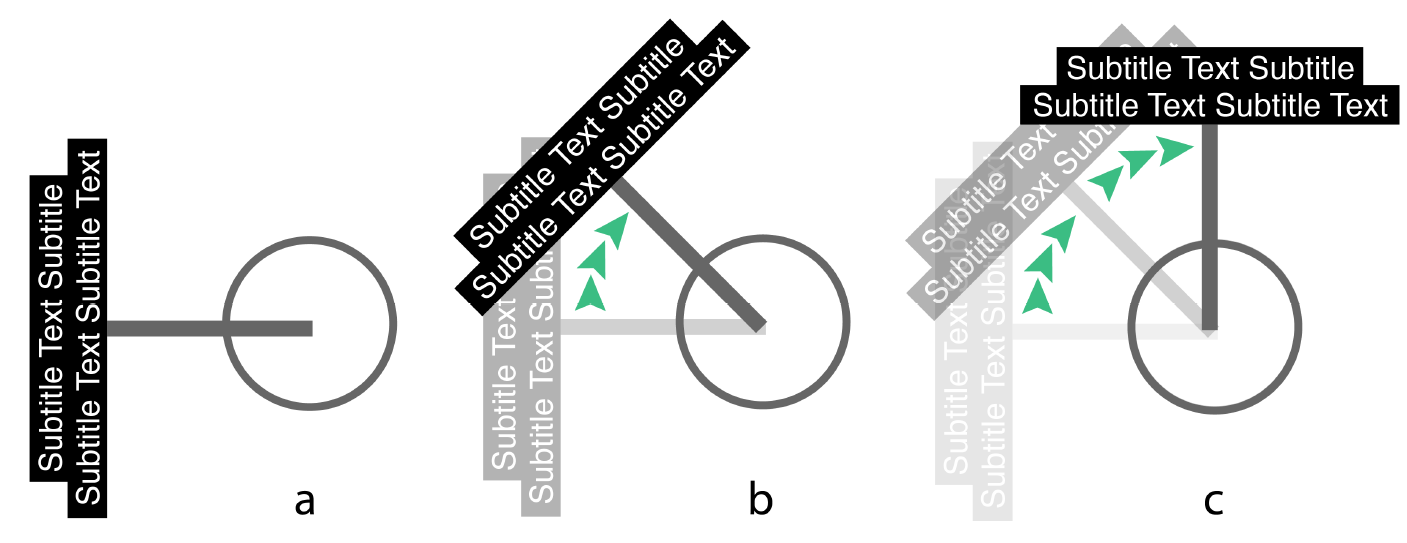
\includegraphics[width=0.7\textwidth]{img/video360/static-follow.png}
    \caption{Static-Follow: The sequence a, b, c demonstrates how as the user turns their head, the subtitles stay fixed to the centre of their field of view. Extracted from the work of Brown et al. (2017).}
    \label{fig:static_follow}
\end{figure}

\subsubsection{Lag-Follow}
\label{subsubsec:lag_follow}

The work of \cite{brown_subtitles_2017} defines the \emph{lag-follow}~(see Figure \ref{fig:lag_follow}) strategy to address the sickness related to the \emph{static-follow} strategy while still keeping the subtitles visible to the viewer. Similar to the \emph{static-follow} strategy, the subtitles appear in front of the viewer. It remains in such position~(relative to the environment) until the viewer's head rotates more than the 30º threshold. The subtitles then smoothly rotates to be in front of the viewer again. It is worth noticing that the subtitles can only move along the horizontal axis. The main objective of this strategy is to provide freedom of movement to the viewer without immediate reaction from subtitles. \cite{brown_subtitles_2017} say, however, that this strategy may cause the viewer to reread the subtitles, which is not desirable.

\begin{figure}[!ht]
    \centering
    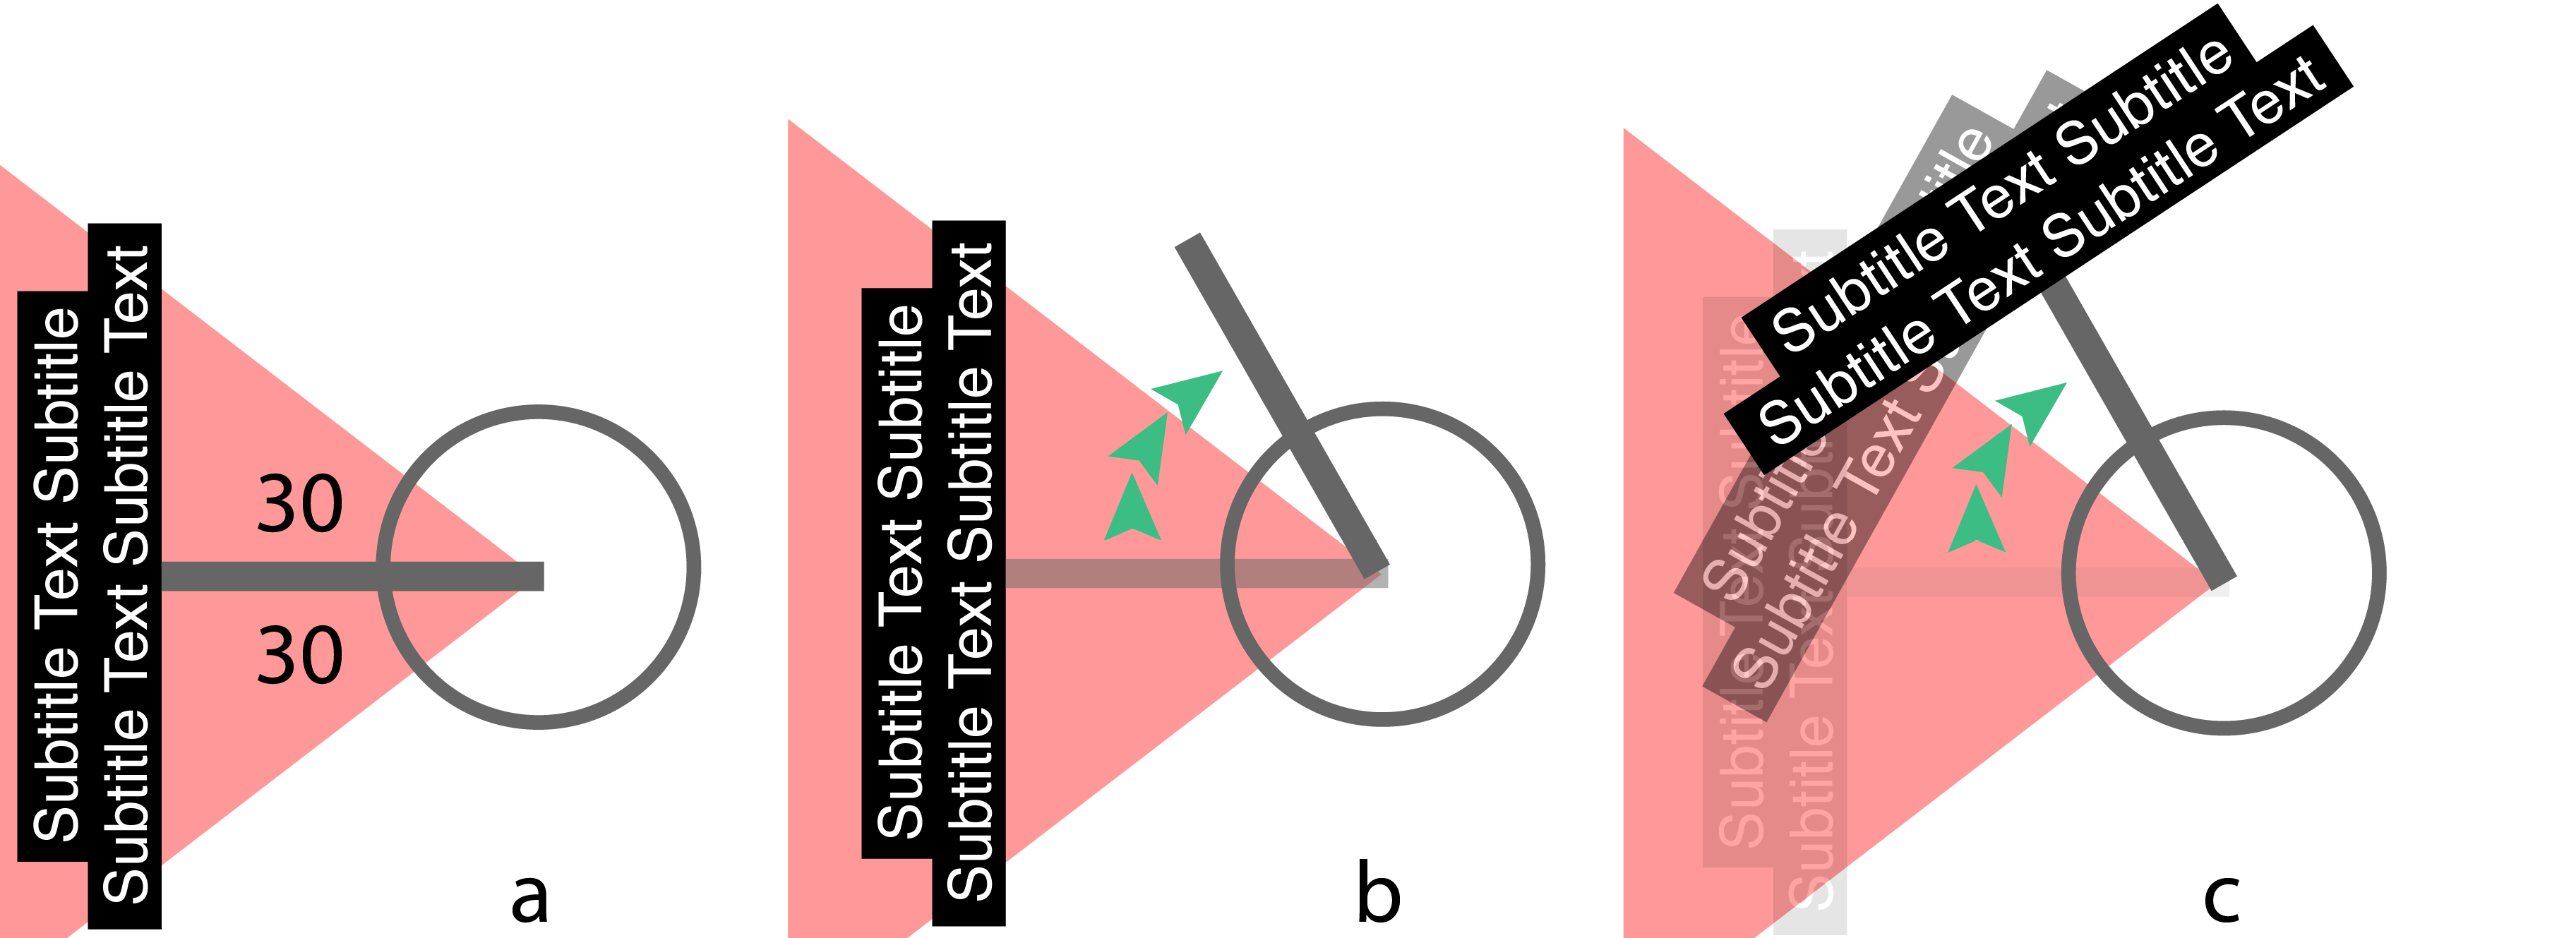
\includegraphics[width=0.7\textwidth]{img/video360/lag-follow.png}
    \caption{Lag-Follow: a. Small user head movements ($<30^{\circ}$) are ignored. b. But turning beyond this boundary c. The subtitles move smoothly to the center of the field-of-view. Extracted from the work of Brown et al. (2017).}
    \label{fig:lag_follow}
\end{figure}

The work of \cite{matos_dynamic_2018} describes a strategy that is basically the same of this one. It is called \emph{floating}, it starts in a position and floats into the viewer's field-of-view. Similar to what was described in Subsection \ref{subsubsec:static_follow}, the work of \cite{montagud_culture_2020} refers to this strategy with a different name (\emph{follow with lag}), but having the same definition.

\subsection{World-Referenced Subtitles}
\label{subsec:world_referenced}

In this category, the subtitles are positioned by taking the 360 environment as reference. 
As referenced in \cite{hughes_disruptive_2019}, this category of strategy leads to better results in comfort~\cite{rothe2018positioning}. \cite{rothe2018positioning}, as referenced in \cite{hughes_disruptive_2019}, also say that world-referenced subtitles conflict, in general, with the requirement that a user must always be able to read the subtitle text because it limitates the user's freedom of exploring the scene.
We have identified two strategies following this category: \emph{repeated subtitles} and \emph{appear subtitles}. These strategies are described in Subsections \ref{subsubsection:repeated_subtitles} and \ref{subsubsection:appear_subtitles}, respectively. 

\subsubsection{Repeated Subtitles}
\label{subsubsection:repeated_subtitles}

In this strategy, repeated subtitles are place around the user. These subtitles stay fixed in the environment and do not follow the user's head motion. Figure \ref{fig:120_subtitles} shows three repeated subtitles evenly spaced by angles of 120°. Such figure was extracted from the work of \cite{brown_subtitles_2017}. The authors argue that one of the main advantages of this strategy for subtitles positioning is that the subtitles could be ``burnt-in'' to the video using a video-editor. This strategy is referenced as \emph{120-degree} in the work of \cite{brown_subtitles_2017}, and as \emph{evenly spaced} in the work of \cite{montagud_culture_2020}. A caveat of this strategy, mentioned by \cite{brown_subtitles_2017}, is that it may cover important content located in unfortunate positions. 

The work of \cite{li_impacts_2018} uses this strategy to evaluate the impacts of subtitles in 360-degree video journalism. They do not evaluate the subtitles positioning itself, but the impact of the subtitles. The work of \cite{chen_film_2017} uses this strategy for positioning subtitles while investigating film language in society news using 360-degree videos of The New York Times. During their study, some participants found the \emph{repeated subtitles} strategy confusing as they thought, in some moments, that the subtitles in different positions had different text.

\begin{figure}[!ht]
    \centering
    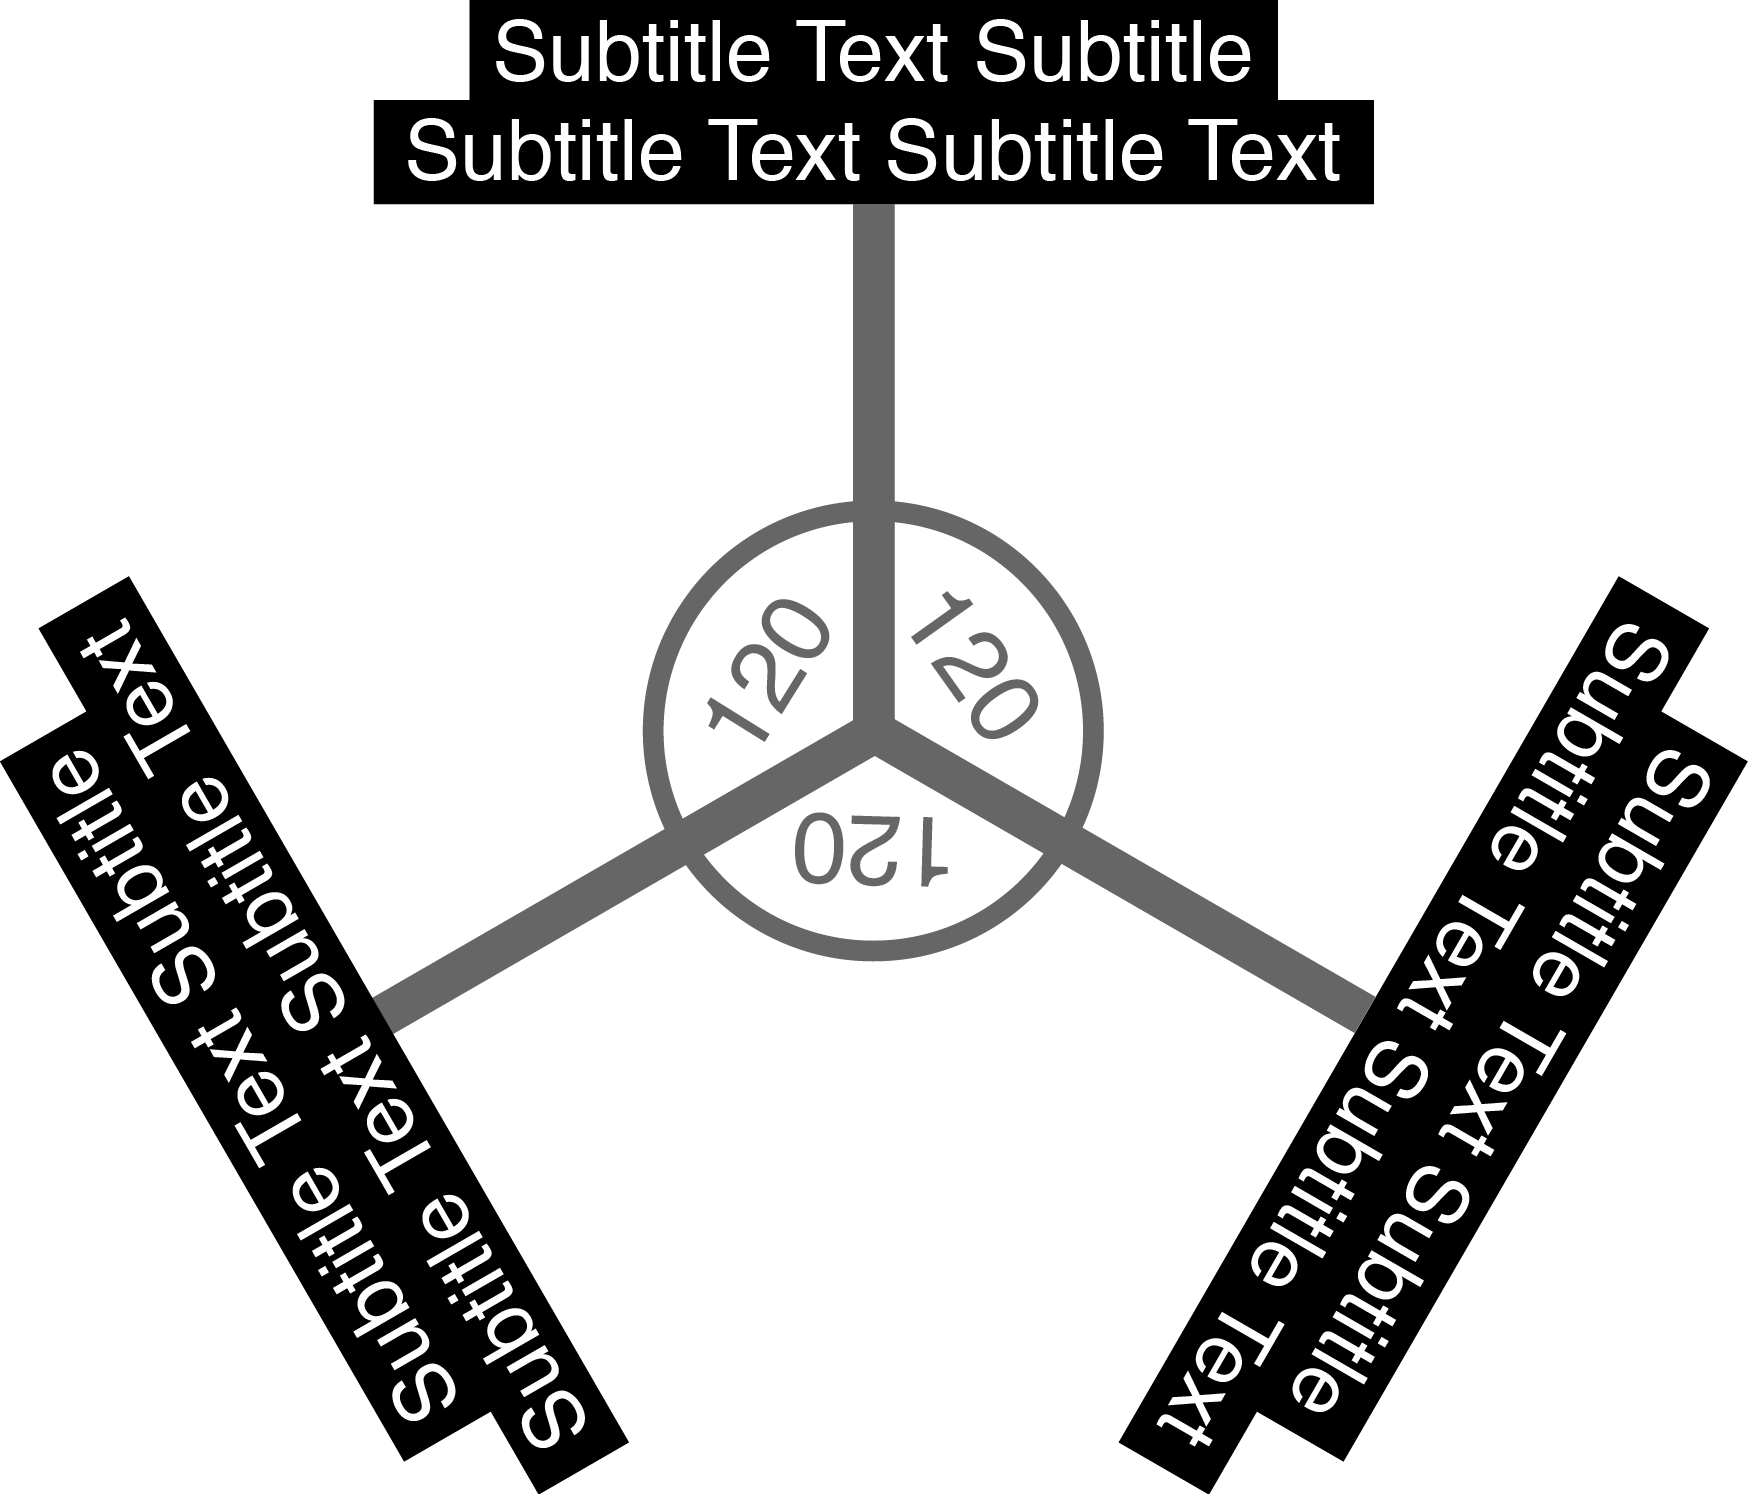
\includegraphics[width=0.35\textwidth]{img/video360/120_subtitles.png}
    \caption{Three repeated subtitles (having the same text) are located in the environment at 120° angles around the viewer. Extracted from the work of Brown et al. (2017).}
    \label{fig:120_subtitles}
\end{figure}


\subsubsection{Appear Subtitles}
\label{subsubsection:appear_subtitles}

\cite{brown_subtitles_2017} say that, based on feedback from a user whom was hard of hearing, they had the idea of creating a strategy in which the viewer can dismiss the subtitle after reading it. From that feedback, they designed the \emph{appear} strategy. As it is depicted in Figure \ref{fig:appear_subtitle}, the subtitles are placed at the centre of the user's field of view horizontally, 15º bellow eye-level. If the viewer moves their head, the subtitles remain static within the environment and do not follow their gaze. This strategy is also referenced as \emph{appear in front, then fixed} in the work of \cite{montagud_culture_2020}. A possible caveat of this strategy, mentioned by \cite{brown_subtitles_2017}, is that the subtitles may be positioned in spurious locations if the viewer is quickly moving their head.

\begin{figure}[!ht]
    \centering
    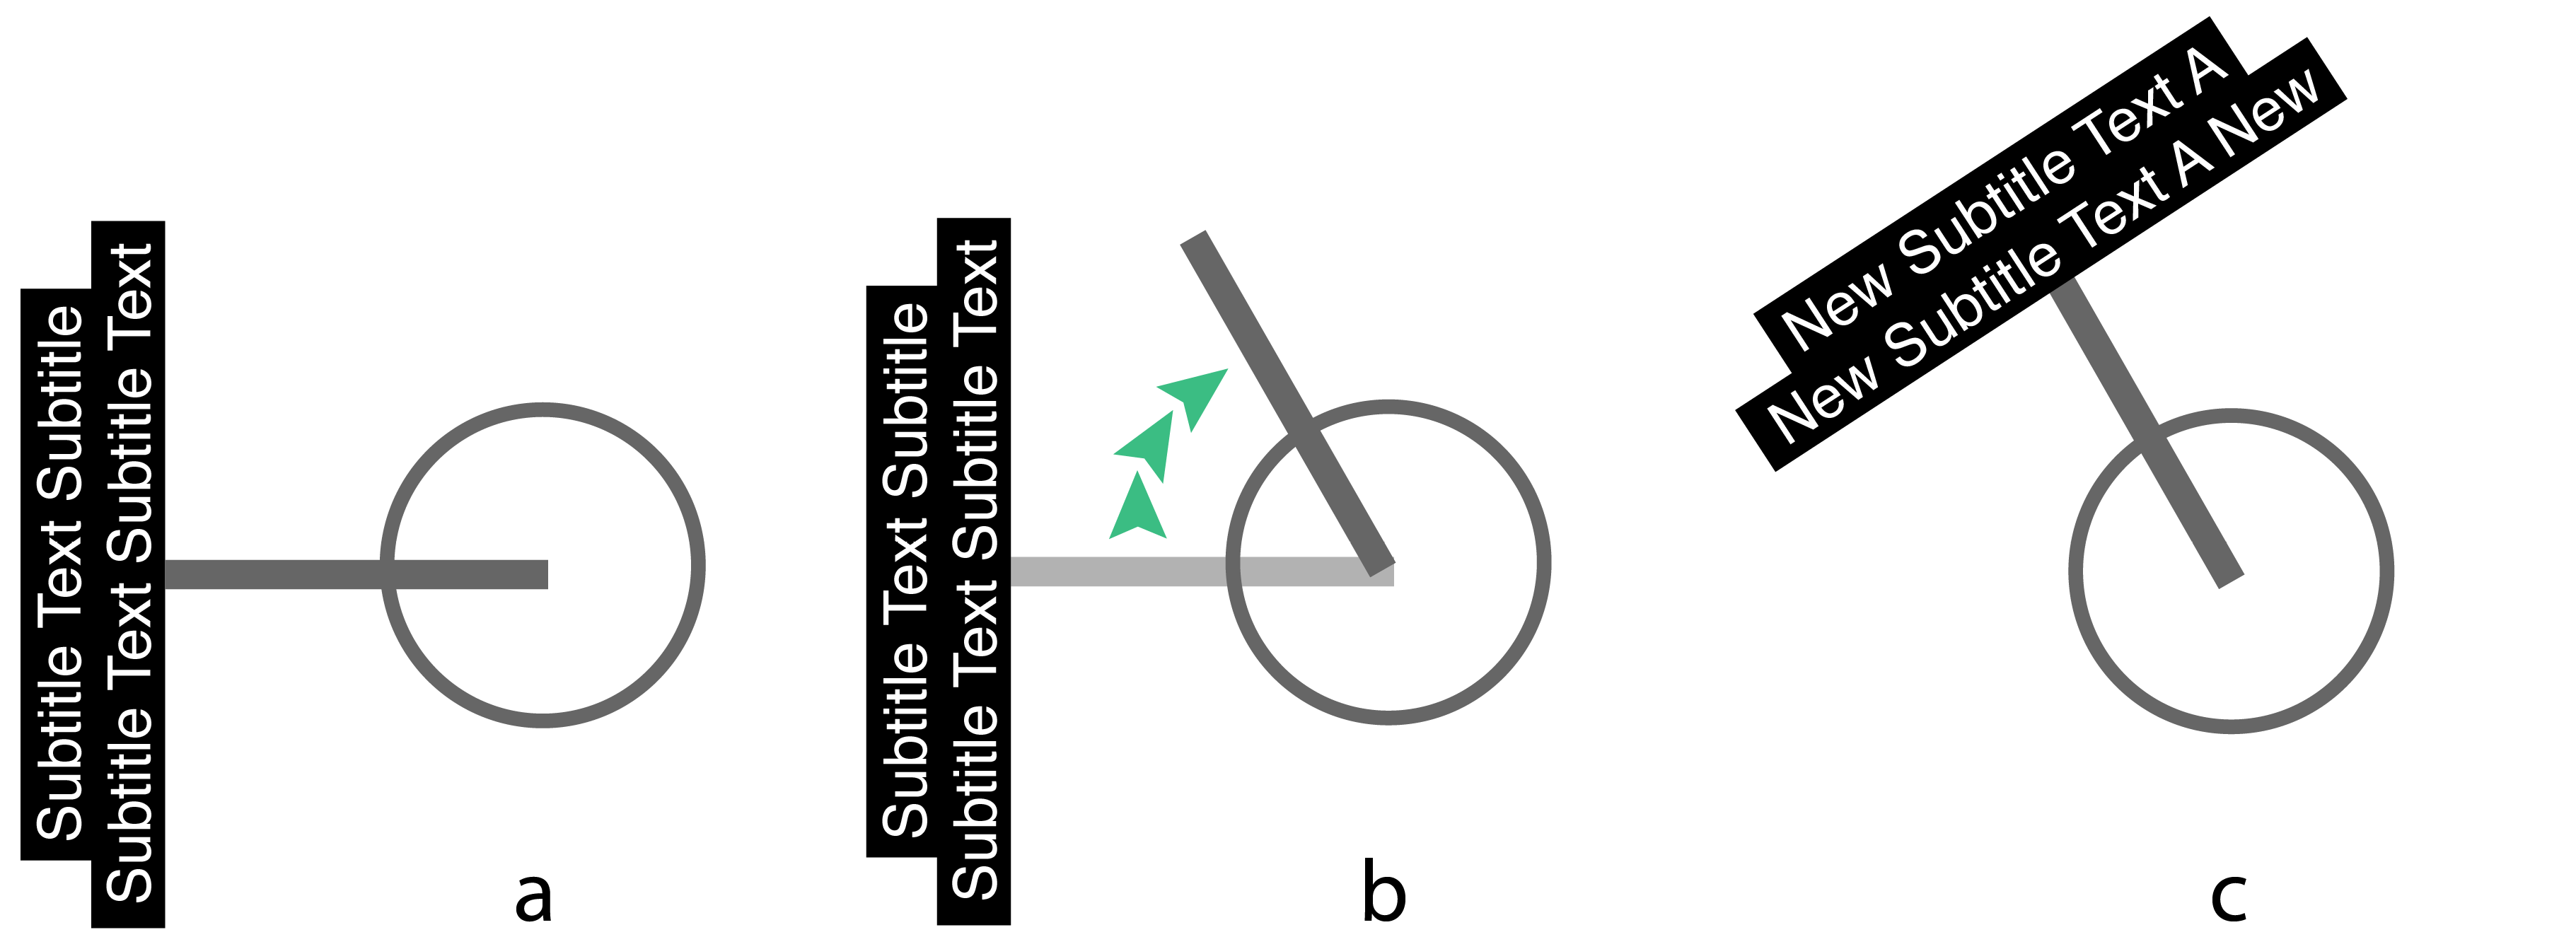
\includegraphics[width=0.7\textwidth]{img/video360/appear.png}
    \caption{Appear: a. A subtitle appears at the centre of the user's view. b. If the user moves before the subtitle is due to change, it will remain static in the environment. c. When a new subtitle is shown, it will appear at the centre of the user's view again. Extracted from the work of Brown et al. (2017).}
    \label{fig:appear_subtitle}
\end{figure}

\subsection{Dynamic Subtitles}
\label{subsection:dynamic_subtitles}

In this category, the position of subtitles dynamically changes and depends on the scene \cite{rothe_dynamic_2018}. As referring to annotations~(that could be subtitles), \cite{matos_dynamic_2018} say that there are cases where the point of interest is moving through the video, which requires a dynamic annotation that follows its movement. One strategy that we have identified in this category is the \emph{speaker-following subtitles} strategy, described in \ref{subsubsec:speaker_following}.

\subsubsection{Speaker-Following Subtitles}
\label{subsubsec:speaker_following}

In this strategy, the subtitles are placed close to the speaker~(see Figure \ref{fig:speaker_following}). Since the speakers may move during the video, this strategy fits in the \emph{dynamic subtitles} category. This strategy also helps in the issue of \emph{speaker identification}, as all persons in the room are visible in a 360-degree video~\cite{rothe_dynamic_2018}.  

\cite{rothe_dynamic_2018} compared \emph{speaker-following} subtitles with the \emph{static-follow} strategy regarding task workload, simulator sickness and presence. For evaluating each of these dimensions, the authors used, respectively, the following questionaires: NASA-TLX~\cite{nasa_hart1988development}; Simulator Sickness Questionaire~\cite{sickness_kennedy1993simulator}; and Presence Questionaire~\cite{presence_witmer1998measuring}. When asking which strategy the participants preferred, the authors received balanced answers. However, \emph{speaker-following} subtitles led to higher score of presence, less sickness and lower workload~\cite{rothe_dynamic_2018}.

\begin{figure}[!ht]
    \centering
    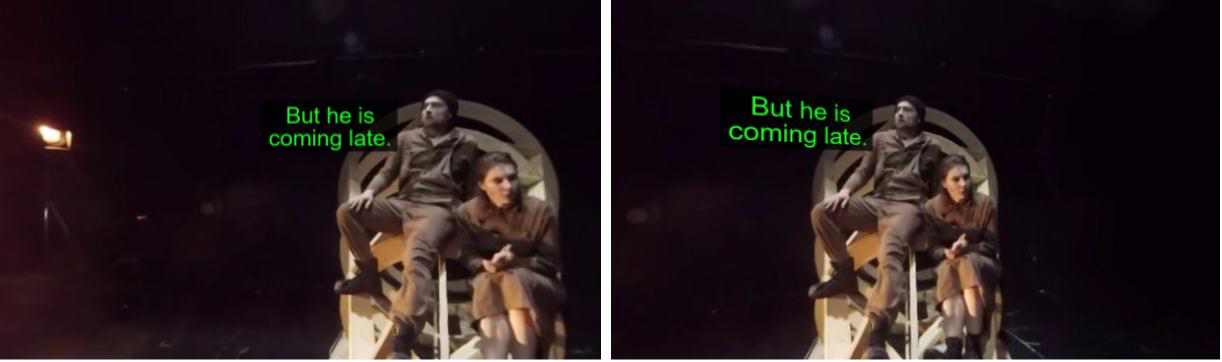
\includegraphics[width=0.95\textwidth]{img/video360/speaker-following.png}
    \caption{Speaker-following subtitles. Extracted from the work of Hughes et al. (2019).}
    \label{fig:speaker_following}
\end{figure}


Similar to the work of \cite{rothe_dynamic_2018}, we intend to position subtitles close to the speakers in the 360-video. The main difference of our work, however, is that we automatically detect the actors present in a 360-video and use their position for placing the subtitles according to an authoring model we propose. In our authoring model, we can also determine the direction that the user is looking at. We use that to position the subtitles as \emph{static-follow} when the actor speaking is not visible to the user. In this way, the disadvantage of \emph{speaker-following} subtitles being not always visible is suppressed.
%%%% -*- coding: utf-8 -*-
\newpage

\chapter{Proposed Approach}
\label{chap:approach}
%%% -*- coding: utf-8 -*-
\newpage

\chapter{Conclusions}
\label{chap:conclusions}

In this dissertation, we present a method for spatio-temporal localization of actors based on \emph{Video Face Clustering}. As part of this method, we also define an algorithm for finding an adequate number of clusters based on the silhouette score. We investigate to what extent this method can be used as the core to leverage and enhance some innovative applications, especially in three different practical and important tasks: \emph{Video Face Recognition}, \emph{Educational Video Recommendation}, and \emph{Subtitles Positioning in 360-Video}.

For the \emph{Video Face Recognition}, we propose a cluster-matching-based approach, derived mainly by the characteristics of our core \emph{Video Face Clustering} method, which is very scalable since the effort spent with annotations is significantly reduced --- as it is done over clusters instead of single images. This method uses \emph{Video Face Clustering} and a heuristic for cluster matching to recognize people in videos. It has achieved a recall of 99.435\% and precision of 99.131\% when considering faces extracted from a set of 13 video files. As another consequence of face clustering, our technique can be useful for creating and labeling datasets in a less time-consuming way by labeling clusters instead of individual images. One of the limitations of this application is related to the size of the video set used for the overall evaluation of our method. This is due to the difficulty of finding videos where it is possible to manually identify in each frame whether each person present is registered or not in our labeled clusters.

For the \emph{Educational Video Recommendation} task, we investigate a new feature that can be used for such recommendation: the presence of specific lecturers, which again is a direct result of the application of our core method. After performing \emph{Video Face Clustering} on each video, we extract their centroids to perform another clustering step that creates a relationship of videos that share the presence of the same lecturers. Finally, we rank the recommended videos based on the amount of time that each lecturer is present. Our method uses only the video files for performing recommendations, no other information about these videos nor the identity of the lecturers is necessary. It is worth mentioning that we do not intend to substitute other video recommendation methods, rather our application shows that, if the presence of lecturers is a relevant feature for educational video recommendation, it can be used for this purpose with a mAP value of 0.99. The main limitation of this application is that we can only recommend videos in which the lecturers are visually present. As future work, we intend to investigate a hybrid recommendation approach, that combines both textual and audiovisual information from the video to create clusters.

For the \emph{Subtitles Positioning in 360-Video} task, our main contribution is the proposal of dynamic placement of subtitles based on the automatic localization of actors. To achieve this goal, we adapted our spatio-temporal localization method to the 360-video setting and created an authoring model for interactive 360-videos. Because of the severe distortions present in equirectangular 360-videos, we used an approach based on viewports extraction for the face detection step of \emph{Video Face Clustering}. To evaluate this approach against the sole use of a traditional CNN, we created a synthetic dataset by projecting images from the FDDB benchmark to equirectangular backgrounds. Our approach, which consists of using viewports with a traditional CNN, performed better than using the traditional CNN directly to the equirectangular images. Moreover, we proposed an authoring model that allows authors to design and create interactive 360 videos. The proposed model is the result of the analysis of different scenarios of immersive 360 multimedia applications. Besides supporting subtitles positioning in 360-videos, it also supports navigation among 360-videos, additional media, etc. 

In summary, we highlight the following contributions of this dissertation:
%%
\begin{enumerate}
    \item A method for video face recognition that is easily scalable and helps in labeling images dataset;
    \item A method for educational video recommendation based on the presence of lecturers;
    \item A method for face detection in equirectangular 360-images that uses models pre-trained with traditional images;
    \item A synthetic dataset for face detection in equirectangular 360-images;
    \item An authoring model for interactive 360-videos;
    \item A player for interactive 360-videos;
    \item An approach for automatic positioning subtitles in 360-videos based on the actors' positions;
\end{enumerate}

The choice for our three proposed applications was due to observations of opportunities to apply \emph{Video Face Clustering} in different contexts. We started with \emph{Video Face Recognition} task. We observed that the use of only the \emph{Video Face Clustering} part of the method could generate the time segments that each actor is present without having to identify them. Then, we hypothesized that this particular feature could also be used to clustering actors in different videos. From this observation, we decided to investigate a method for \emph{Educational Video Recommendation} using this clustering of actors in different videos. The idea for \emph{Subtitles Positioning in 360-video} came from the authoring model we developed. We observed that we could automatically identify the actors using \emph{Video Face Clustering} so that the subtitles could follow the speakers in the 360-video. Thus, we adapted \emph{Video Face Clustering} for the 360-video setting. It is worth noticing that with this adaptation, the other two applications~(\emph{Video Face Recognition} and \emph{Educational Video Recommendation}) could also be applied to the context of 360-videos.

This work has opened lots of branches for future research. For the particular case of subtitles positioning in 360-video, there is still much to explore. It is not yet clear what is the most adequate way to place subtitles relative to the actors' positions. For instance: is it better to place them above or below the actors' faces? Should the subtitles follow the actors immediately or it would be better to have a delay with a smooth transition? A path towards answering these questions is by experimenting and evaluating these and other possible settings with users.

Other possible future work comes from the combination of the applications we explored in this dissertation. For instance, the identification of lecturers using a lecturer's image dataset with \emph{Video Face Recognition} could improve the task of \emph{Educational Video Recommendation} by inserting additional relationships among lecturers~(e.g. lecturers that teach the same subject). Another possibility is to use \emph{Video Face Recognition} to identify and insert the name of the actor present in 360-videos together with the subtitles so that the users know who is talking when the actor is not visible to them.

Although this dissertation has focused on faces, the methods and techniques here investigated could also be applied in other contexts. For instance, we could recommend videos based on the presence of the same \emph{actions} in different videos, so that a reference video with many actions related to culinary, for example, such as pouring and chopping should have videos with similar \emph{actions} as recommended. For doing that, we should be able to represent each action identified as an embedding~(vector). Then, the remainder of our method for \emph{Educational Video Recommendation} could be used. In the context of 360-videos, if we could generate art embeddings from pieces of art, we could apply the process of \emph{Video Face Clustering}~(or \emph{Video Art Clustering} in this case) to detect and determine the video segments that each piece of art is present. In this case, instead of using \emph{CNNs} trained for detecting and generating embeddings for faces, we would use them for pieces of art. By doing that, we would be able to use our authoring model to attach additional media such as text and audio to pieces of art in an interactive 360-video. This application could be useful in the context of virtual tours in museums and historical sites.


\section{Publications}

 As a result of this research, three papers have already been published at relevant multimedia conferences \cite{mendes2020cluster,mendes2020ISM, mendes2020authoring}. In \cite{mendes2020cluster}, we have evaluated video face clustering together with a cluster-matching method for video face recognition. In \cite{mendes2020ISM}, we have used video face clustering and the presence of actors in different videos as a means for recommending educational videos. In \cite{mendes2020authoring}, we have developed an authoring model and a player for interactive 360-video. 

\arial
\bibliography{references}

% Apendix chapters below.
%\normalfont
%\appendix
%\newpage

\chapter{User profile questionnaire for prototype evaluation sessions}
\label{chap:profile-form}

\begin{enumerate}
\item Personal information
  \begin{enumerate}
 \item Name
 \newline \rule[0pt]{300pt}{1pt}
 \item E-mail
 \newline \rule[0pt]{300pt}{1pt}
 \item Education degree
 \newline \rule[0pt]{300pt}{1pt}
 \item Course semester (just for students)
 \newline \rule[0pt]{300pt}{1pt}
 \item Occupation
 \newline \rule[0pt]{300pt}{1pt}
  \end{enumerate}
\item Please mark below your knowledge about the following subjects:
	\begin{enumerate}
   \item Division of a sample by percentiles: P10, P50, P80 ...
		\newline \circle{10} I do not know
     \newline \circle{10} I know little (I have learned these concepts at some point, but may have to learn again if I have to apply them)
     \newline \circle{10} I have average knowledge (I may have to revise one concept or another if I have to apply it)
     \newline \circle{10} I know well (I do not apply often, but I would not need to revise the concepts if I had to apply them)
     \newline \circle{10} I am a specialist (I apply these concepts frequently)
	  \newline 
   \item Analysis of trends and patterns in time series
   \newline \circle{10} I do not know
   \newline \circle{10} I know little (I have learned these concepts at some point, but may have to learn again if I have to apply them)
   \newline \circle{10} I have average knowledge (I may have to revise one concept or another if I have to apply it)
   \newline \circle{10} I know well (I do not apply often, but I would not need to revise the concepts if I had to apply them)
   \newline \circle{10} I am a specialist (I apply these concepts frequently)\\
      
   \item Projection chart (Time-lapsed LAMP chart)
   \begin{figure}[H]
		\centering
		\includegraphics[width=0.9\columnwidth]{images/form-timelapsedchart.png}
		\label{fig:form-timelapsedchart}
	   \end{figure}

   \circle{10} I do not know
   \newline \circle{10} I know little (I have learned these concepts at some point, but may have to learn again if I have to apply them)
   \newline \circle{10} I have average knowledge (I may have to revise one concept or another if I have to apply it)
   \newline \circle{10} I know well (I do not apply often, but I would not need to revise the concepts if I had to apply them)
   \newline \circle{10} I am a specialist (I apply these concepts frequently)\\

 \newpage
       \item Ranking chart (Bump chart)
       \begin{figure}[H]
 		\centering
 		\includegraphics[width=0.9\columnwidth]{images/form-bumpchart.png}
 		\label{fig:form-bumpchart}
 	   \end{figure}
       
       \circle{10} I do not know
       \newline \circle{10} I know little (I have learned these concepts at some point, but may have to learn again if I have to apply them)
       \newline \circle{10} I have average knowledge (I may have to revise one concept or another if I have to apply it)
       \newline \circle{10} I know well (I do not apply often, but I would not need to revise the concepts if I had to apply them)
       \newline \circle{10} I am a specialist (I apply these concepts frequently)\\

 \newpage
       \item Distance chart
       \begin{figure}[H]
 		\centering
 		\includegraphics[width=0.9\columnwidth]{images/form-distancechart.png}
 		\label{fig:form-distancechart}
 	   \end{figure}
      
       \circle{10} I do not know
       \newline \circle{10} I know little (I have learned these concepts at some point, but may have to learn again if I have to apply them)
       \newline \circle{10} I have average knowledge (I may have to revise one concept or another if I have to apply it)
       \newline \circle{10} I know well (I do not apply often, but I would not need to revise the concepts if I had to apply them)
       \newline \circle{10} I am a specialist (I apply these concepts frequently)\\

 \newpage
       \item Fanchart
       \begin{figure}[H]
 		\centering
 		\includegraphics[width=0.9\columnwidth]{images/form-fanchart.png}
 		\label{fig:form-fanchart}
 	  \end{figure}
      
       \circle{10} I do not know
       \newline \circle{10} I know little (I have learned these concepts at some point, but may have to learn again if I have to apply them)
       \newline \circle{10} I have average knowledge (I may have to revise one concept or another if I have to apply it)
       \newline \circle{10} I know well (I do not apply often, but I would not need to revise the concepts if I had to apply them)
       \newline \circle{10} I am a specialist (I apply these concepts frequently)

     \end{enumerate}
\end{enumerate}

\bibliographystyle{bibstyles/abnt-alf}

\end{document}